\documentclass{article}
\usepackage[a4paper, margin=1in]{geometry}
\usepackage{amsmath} % for math
\usepackage{enumerate} % for items
\usepackage{verbatim} % for code
\usepackage{graphicx} % for images
\usepackage{hyperref} % for links

% To include an image, use the following command:
% \includegraphics[width=Xcm]{file.extension}
% where X = integer

\title{COMP 3005 Project}
\author{Nicolas El-Khoury, Vinh Nguyen}
\date{April 14, 2020}

\begin{document}
    \maketitle

    \section{Conceptual Design}

        \subsection{Assumptions}
    
        Book:
        \begin{itemize}
            \item Each book's ISBN must be unique.
            \item Books may have the same title, author, and genre.
            \item The same book can be published by different publishers.
        \end{itemize}
        
        \noindent User:
        \begin{itemize}
            \item Each username must be unique.
            \item Users may have the same email, address, and phone number.
            \item Genders are restricted to $\{m, f, o\}$, representing 'Male', 'Female', and 'Other'.
        \end{itemize}
        
        \noindent Publisher:
        \begin{itemize}
            \item Publishers may have the same name, banking account, address, email, and phone number.
        \end{itemize}
        
        \noindent Order:
        \begin{itemize}
            \item Orders must have unique IDs and may only have one corresponding user.
            \item Orders may have the same date, tracking number, shipping company, billing and shipping address, and payment method.
        \end{itemize}
        
        \noindent Address:
        \begin{itemize}
            \item Addresses may have the same street number, street name, city, province, and postal code.
        \end{itemize}
        
        \noindent Store:
        \begin{itemize}
            \item Each store only has one owner.
            \item Each store requires a corresponding user.
            \item Different stores may contain the same book(s).
        \end{itemize}
        
        \subsection{ER Diagram}
    
        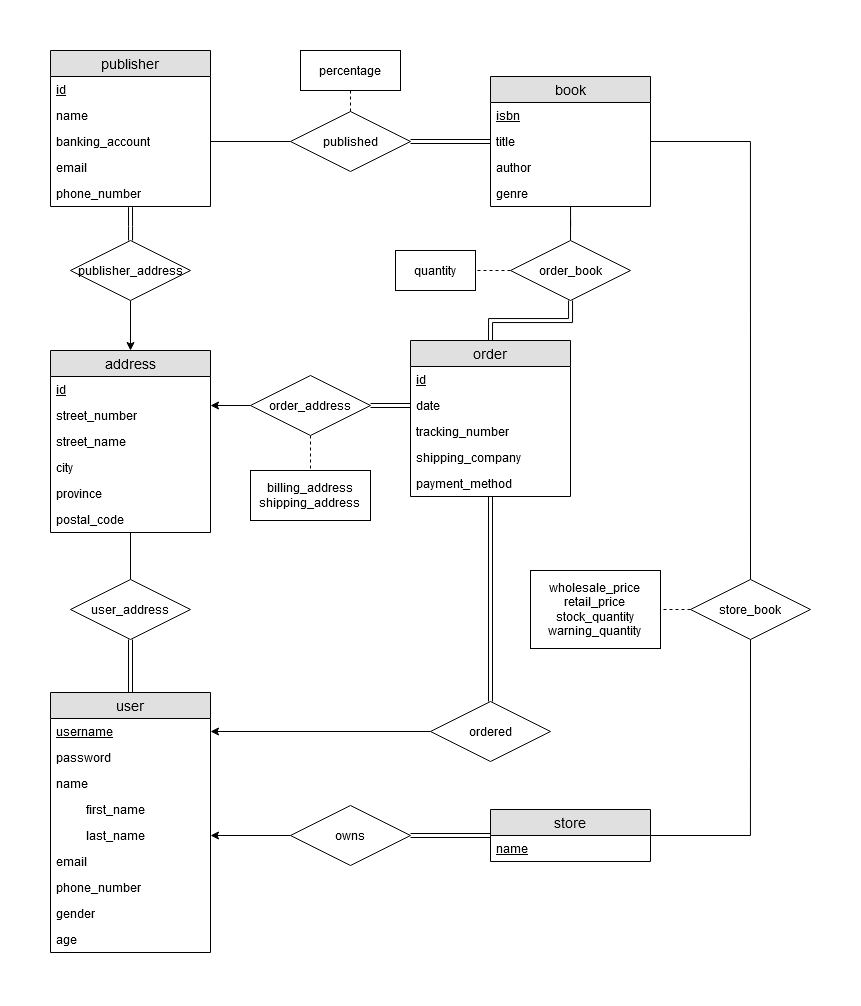
\includegraphics[width=16cm]{er-diagram_current.png}

    \section{Reduction to Relation Schemas}

    \begin{itemize}
        \item book(\underline{isbn}, title, author, genre)
        \item publisher(\underline{id}, publisher\_name, banking\_account, address\_id, email, phone\_number) \emph{foreign key (address\_id) references address(id)}
        \item published(\underline{isbn}, \underline{publisher\_id}, pub\_percentage)
        \item address(\underline{id}, street\_number, street\_name, city, province, postal\_code)
        \item order(\underline{id}, date, tracking\_number, shipping\_company, billing\_address, shipping\_address, payment\_method) \emph{foreign key (billing\_address) references address (id), foreign key (shipping\_address) references address(id)}
        \item user(\underline{username}, password, first\_name, last\_name, address\_id, email, phone\_number, gender, age) \emph{foreign key (address\_id) references address(id)}
        \item store(\underline{store\_name}, \underline{username}) \emph{foreign key (username) references user(username)}
        \item store\_books(\underline{store\_name}, \underline{isbn}, retail\_price, wholesale\_price, stock\_quantity, warning\_quantity) \emph{foreign key (username) references user(username), foreign key (isbn) references book(isbn)}
        \item ordered(\underline{order\_id}, username) \emph{foreign key (order\_id) references order(id), foreign key (username) references user(username)}
        \item order\_book(\underline{order\_id}, \underline{isbn}, quantity) \emph{foreign key (order\_id) references order(id), foreign key (isbn) references book(isbn)}
    \end{itemize}

    \section{Normalization of Relation Schemas}
    
    \subsection{Book}
    
    isbn $\rightarrow$ title, author, genre, publisher\_percentage \\
    isbn $\rightarrow$ title, author, genre, publisher\_percentage, isbn (Axiom of Augmentation) \\
    (isbn)$^+$ = \{title, author, genre, publisher\_percentagem, isbn\} \\
    
    \noindent Since the LHS of our functional dependency is our super key, and it is a non-trivial functional dependency, the book relation is currently in BCNF since there are no violations.

    \subsection{Publisher}
    publisher\_id $\rightarrow$ publisher\_name, banking\_account, address, email, phone\_number \\
    publisher\_id $\rightarrow$ publisher\_name, banking\_account, address, email, phone\_number, publisher\_id (Axiom of Augmentation) \\
    (publisher\_id)$^+$ = \{publisher\_name, banking\_account, address, email, phone\_number, publisher\_id\} \\
    \noindent Since every LHS on the functional dependency is a candidate key, and all of the functional dependencies are non-trivial, the publisher relation is currently in BCNF since there are no violations.
    
    \subsection{Published}
    
    \noindent isbn, publisher\_id $\rightarrow$ pub\_percentage \\
    \noindent isbn, publisher\_id $\rightarrow$ pub\_percentage, isbn, publisher\_id (Axiom of Augmentation) \\
    (isbn, publisher\_id)$^+$ = \{pub\_percentage, isbn, publisher\_id\} \\
    
    \noindent Since the LHS of our functional dependency is our super key, and it is a non-trivial functional dependency, the published relation is currently in BCNF since there are no violations.
    
    \subsection{Order}
    id $\rightarrow$ date, tracking\_number, shipping\_company, billing\_address, shipping\_address, payment\_method \\
    id $\rightarrow$ date, tracking\_number, shipping\_company, billing\_address, shipping\_address, payment\_method, id (Axiom of Augmentation)\\
    (id)$^+$ = \{date, tracking\_number, shipping\_company, billing\_address, shipping\_address, payment\_method, id\} \\
    
    \noindent Since the LHS of our functional dependency is our super key, and it is a non-trivial functional dependency, the order relation is currently in BCNF since there are no violations. \\
    
    \subsection{User}
    username $\rightarrow$ password, first\_name, last\_name, address\_id, email, phone\_number, gender, age \\
    username $\rightarrow$ password, first\_name, last\_name, address\_id, email, phone\_number, gender, age, username (Axiom of Augmentation)\\
    (username)$^+$ = \{password, first\_name, last\_name, address\_id, email, phone\_number, gender, age, username\} \\
    \noindent Since the LHS of our functional dependency is our super key, and it is a non-trivial functional dependency, the user relation is currently in BCNF since there are no violations. \\
    
    \subsection{Store}
    username $\rightarrow$ store\_name \\
    store\_name $\rightarrow$ username \\
    username $\rightarrow$ store\_name, username (Axiom of Augmentation) \\
    store\_name $\rightarrow$ username, store\_name (Axiom of Augmentation) \\
    (username)$^+$ = \{store\_name, username\} \\
    (store\_name)$^+$ = \{username, store\_name\} \\
    
    \noindent Since the LHS of our functional dependencies are super keys, and they are non-trivial functional dependencies, the store relation is currently in BCNF since there are no violations. \\
    
    \subsection{Store\_books}
    store\_name, isbn $\rightarrow$ retail\_price, wholesale\_price, stock\_quantity, warning\_quantity \\
    store\_name, isbn $\rightarrow$ retail\_price, wholesale\_price, stock\_quantity, warning\_quantity, store\_name, isbn (Axiom of Augmentation) \\
    (store\_name, isbn)$^+$ = \{retail\_price, wholesale\_price, stock\_quantity, warning\_quantity, store\_name, isbn\} \\
    
    \noindent Since the LHS of our functional dependency is our super key, and it is a non-trivial functional dependency, the store\_books relation is currently in BCNF since there are no violations. \\
    
    \subsection{Ordered}
    order\_id $\rightarrow$ username \\
    order\_id $\rightarrow$ username, order\_id (Axiom of Augmentation) \\
    (order\_id)$^+$ = \{username, order\_id\} \\
    
    \noindent Since the LHS of our functional dependency is our super key, and it is a non-trivial functional dependency, the ordered relation is currently in BCNF since there are no violations. \\
    
    \subsection{Order\_book}
    order\_id, isbn $\rightarrow$ quantity \\ 
    order\_id, isbn $\rightarrow$ quantity, order\_id, isbn (Axiom of Augmentation) \\
    (order\_id, isbn)$^+$ = \{order\_id, isbn, quantity\} \\
    
    \noindent Since the LHS of our functional dependency is our super key, and it is a non-trivial functional dependency, the order\_book relation is currently in BCNF since there are no violations. \\
    
    \subsection{Address}
    id $\rightarrow$ street\_number, street\_name, city, province, postal\_code \\
    id $\rightarrow$ street\_number, street\_name, city, province, postal\_code, id (Axiom of Augmentation) \\
    postal\_code $\rightarrow$ city, province (Axiom of Transitivity) \\
    postal\_code $\rightarrow$ city, province, postal\_code (Axiom of Augmentation) \\
    (id)$^+$ = \{street\_number, street\_name, city, province, postal\_code, id\}
    (postal\_code)$^+$ = \{city, province, postal\_code\} \\
    
    \noindent As we can see, the postal\_code functional dependency violates BCNF. If we decompose address into $R_1$ = (id, postal\_code, street\_number, street\_name), $R_2$ = (postal\_code, city, province), we can maintain BCNF in this decomposed relation.
    
    \section{Database Schema Diagram}
    
    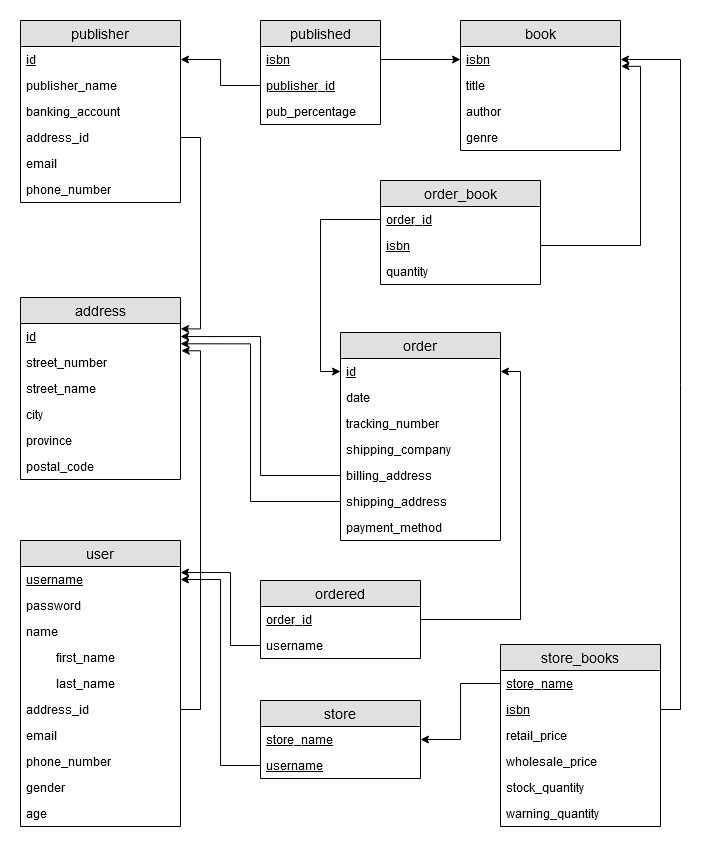
\includegraphics[width=16cm]{schema-diagram_current.png}

    \section{Implementation}

    \subsection{Backend by Nicolas}
    
    Implemented the back-end in NodeJS using the express, pg, and uuidv4 node modules. Creates queries dynamically in order to serve the user the correct information. Acts as a layer between the client and the SQL database that enables interaction in a safe and competent manner. Implements SQL injection protection to ensure users cannot manipulate SQL database in unwanted fashion. Authenticates users on a secure basis, utilizing uuidv4 to generate random authentication keys for each user. They are then verified through routes that utilize SQL queries to the database to ensure the client has the proper authentication levels to access the content they want.
    
    \subsection{Frontend by Vinh}
    
    The frontend is implemented using Node.js with Express, Pug, Axios, and Session modules. Sets up various routes for clients through Express. Serves templated pages to users by using the Pug template engine, based on criteria such as route, authentication, etc. Axios allows the frontend server to communicate with our backend by making XMLHttpRequests serverside to obtain information such as books, users, purchases, management, etc. The session module helps us to implement authentication with users as well as login and logout features for our website.
    
    \subsection{UI Screenshots}
    
    \noindent UI screenshots can be found within our github repository's README, found in \hyperref[sec:github]{section 7}.

    \section{Bonus Features}

    \begin{itemize}
        \item Separate backend and frontend servers, giving us modularity for additional projects and reuse in the future.
        \item Backend server is built as a stateless API, allowing other services and servers to make requests and interact with our database.
        \item Backend dynamically creates query based on given parameters, allowing for reuse with different databases, regardless of structure.
        \item Backend queries use both partial and exact matching for specific cases, allowing for flexibility in our search system.
        \item Frontend is built using Bootstrap for both web and mobile responsiveness, shown in UI screenshots.
        \item Frontend pages differ based on authentication level of client (ex: logged out, logged in, manager).
        \item Frontend has hidden account pages tailored to each user, using template engines and sessions.
    \end{itemize}

    \section{Github Repository}
    \label{sec:github}

    Our project is hosted at the following public repository
    \begin{verbatim}
https://github.com/vinhvn/online-bookstore
    \end{verbatim}

\end{document}